\documentclass[aspectratio=169,12pt]{beamer}

\PassOptionsToPackage{table}{xcolor}

\usepackage[T2A]{fontenc}
\usepackage[utf8]{inputenc}
\usepackage[main=russian,english]{babel}
\usepackage{graphicx}
\usepackage{booktabs}
\usepackage{tabularx}
\usepackage{amsmath}
\usepackage{tikz}
\usepackage{colortbl}
\usepackage{calc}

\usetikzlibrary{shapes.geometric,positioning,calc,arrows.meta}

% ── Images path ──────────────────────────────────────────────
\graphicspath{{../overleaf-sync/images/}}

% ── Color palette ────────────────────────────────────────────
\definecolor{accent}{HTML}{2563EB}      % blue-600
\definecolor{accentlight}{HTML}{DBEAFE} % blue-100
\definecolor{accentmid}{HTML}{93C5FD}   % blue-300
\definecolor{textmain}{HTML}{1E293B}    % slate-800
\definecolor{textsub}{HTML}{64748B}     % slate-500
\definecolor{surfacebg}{HTML}{FFFFFF}   % white
\definecolor{surfacealt}{HTML}{F8FAFC}  % slate-50
\definecolor{ruleclr}{HTML}{E2E8F0}     % slate-200
\definecolor{successclr}{HTML}{16A34A}  % green-600
\definecolor{dangerclr}{HTML}{DC2626}   % red-600
\definecolor{warnclr}{HTML}{D97706}     % amber-600

% ── Theme: stripped-down, light ──────────────────────────────
\usetheme{default}
\setbeamersize{text margin left=10mm,text margin right=10mm}
\setbeamercolor{background canvas}{bg=surfacebg}
\setbeamercolor{normal text}{fg=textmain}
\setbeamercolor{frametitle}{fg=textmain}
\setbeamercolor{structure}{fg=accent}
\setbeamercolor{itemize item}{fg=accent}
\setbeamercolor{itemize subitem}{fg=accentmid}
\setbeamercolor{alerted text}{fg=dangerclr}
\setbeamercolor{block title}{fg=surfacebg,bg=accent}
\setbeamercolor{block body}{bg=accentlight}

\setbeamertemplate{navigation symbols}{}
\setbeamertemplate{footline}{}
\setbeamertemplate{headline}{}
\setbeamertemplate{itemize item}{\textcolor{accent}{\raisebox{0.18ex}{\tiny\textbullet}}}
\setbeamertemplate{itemize subitem}{\textcolor{accentmid}{\raisebox{0.18ex}{\tiny\textbullet}}}

% ── Fonts ────────────────────────────────────────────────────
\setbeamerfont{frametitle}{size=\LARGE,series=\bfseries}
\setbeamerfont{framesubtitle}{size=\normalsize,series=\mdseries}
\setbeamerfont{title}{size=\huge,series=\bfseries}
\setbeamerfont{subtitle}{size=\large,series=\mdseries}
\setbeamerfont{author}{size=\normalsize}
\setbeamerfont{institute}{size=\small}
\setbeamerfont{date}{size=\small}
\setbeamerfont{normal text}{size=\normalsize}

% ── Custom frame title with accent rule ──────────────────────
\setbeamertemplate{frametitle}{%
  \vskip4pt%
  \usebeamerfont{frametitle}\usebeamercolor[fg]{frametitle}\insertframetitle%
  \ifx\insertframesubtitle\empty\else%
    \\[2pt]{\usebeamerfont{framesubtitle}\textcolor{textsub}{\insertframesubtitle}}%
  \fi%
  \vskip3pt%
  \textcolor{accent}{\rule{2.8cm}{2pt}}\textcolor{ruleclr}{\rule{\dimexpr\textwidth-2.8cm}{0.5pt}}%
  \vskip4pt%
}

% ── Slide number (bottom-right, subtle) ──────────────────────
\setbeamertemplate{footline}{%
  \hfill\textcolor{textsub}{\footnotesize\insertframenumber\kern12pt}\vskip6pt%
}

% ── Metadata ─────────────────────────────────────────────────
\title{Обучение с подкреплением\\[4pt]для игры <<Змейка>>}
\subtitle{Курсовая работа}
\author{Полегина~А.\,Д.\\[2pt]{\small Научный руководитель: к.\,ф.-м.\,н., доцент С.\,Г.\,Красовский}}
\institute{БГУ, мехмат, кафедра дифференциальных уравнений и системного анализа}
\date{Минск, 2026}

% ── Helper: accent tag ───────────────────────────────────────
\newcommand{\accenttag}[1]{%
  \tikz[baseline=(t.base)]{\node[fill=accentlight,rounded corners=3pt,inner sep=4pt](t){\textcolor{accent}{\small\bfseries #1}};}%
}
\newcommand{\successtag}[1]{%
  \tikz[baseline=(t.base)]{\node[fill=green!8,rounded corners=3pt,inner sep=4pt](t){\textcolor{successclr}{\small\bfseries #1}};}%
}
\newcommand{\dangertag}[1]{%
  \tikz[baseline=(t.base)]{\node[fill=red!8,rounded corners=3pt,inner sep=4pt](t){\textcolor{dangerclr}{\small\bfseries #1}};}%
}

% ── Card box ─────────────────────────────────────────────────
\newcommand{\card}[2]{%
  \begin{tikzpicture}
    \node[draw=ruleclr,rounded corners=6pt,fill=surfacealt,inner sep=10pt,text width=#1,align=left](c){#2};
  \end{tikzpicture}%
}

\begin{document}

% ═══════════════════════════════════════════════════════════════
%  SLIDE 1 — Title
% ═══════════════════════════════════════════════════════════════
\begin{frame}[plain]
\begin{tikzpicture}[remember picture,overlay]
  % subtle top-right accent blob
  \fill[accentlight] ([xshift=-3cm,yshift=1cm]current page.north east)
    circle[radius=4cm];
  \fill[accent,opacity=0.07] ([xshift=-1cm,yshift=-0.5cm]current page.north east)
    circle[radius=2.5cm];
\end{tikzpicture}
\vfill
\begin{flushleft}
  \hspace{0.8cm}%
  \begin{minipage}{0.8\textwidth}
    \usebeamerfont{title}\usebeamercolor[fg]{normal text}\inserttitle\\[12pt]
    \textcolor{accent}{\rule{3cm}{2.5pt}}\\[14pt]
    \usebeamerfont{author}\insertauthor\\[10pt]
    \usebeamerfont{institute}\textcolor{textsub}{\insertinstitute}\\[6pt]
    \usebeamerfont{date}\textcolor{textsub}{\insertdate}
  \end{minipage}
\end{flushleft}
\vfill
\end{frame}

% ═══════════════════════════════════════════════════════════════
%  SLIDE 2 — Goal & Tasks
% ═══════════════════════════════════════════════════════════════
\begin{frame}{Цель и задачи}

\textbf{Цель:} разработать игру <<Змейка>> на Python, реализовать Q-learning для управления агентом и оценить качество обучения.

\vspace{0.5cm}
\begin{columns}[T]
\column{0.55\textwidth}
\textcolor{textsub}{\small ЗАДАЧИ}
\vspace{0.15cm}
\begin{itemize}
    \setlength\itemsep{0.3cm}
    \item Изучить алгоритм Q-learning
    \item Реализовать логику игры и RL-среду
    \item Задать состояние, действия и награду
    \item Провести эксперименты
\end{itemize}

\column{0.40\textwidth}
\card{0.85\linewidth}{%
  \textcolor{textsub}{\small ПОЧЕМУ <<ЗМЕЙКА>> + RL}\\[6pt]
  \accenttag{Дискретная среда}\\[4pt]
  \accenttag{Мало действий}\\[4pt]
  \accenttag{Наглядный результат}%
}
\end{columns}
\end{frame}

% ═══════════════════════════════════════════════════════════════
%  SLIDE 3 — Approach Comparison
% ═══════════════════════════════════════════════════════════════
\begin{frame}[t,shrink=10]{Сравнение подходов}

\centering
\renewcommand{\arraystretch}{1.25}
\begin{tabularx}{0.94\textwidth}{>{\raggedright\arraybackslash}p{0.22\textwidth} >{\raggedright\arraybackslash}p{0.28\textwidth} X}
    \arrayrulecolor{ruleclr}
    \toprule
    \textcolor{textsub}{\small Подход} & \textcolor{textsub}{\small Плюсы} & \textcolor{textsub}{\small Минусы} \\
    \midrule
    Правила и эвристики & Простота реализации & Слабая адаптивность \\
    Поиск траектории & Явный маршрут & Нет обучения на опыте \\
    \rowcolor{accentlight} \textcolor{accent}{\textbf{Табличный Q-learning}} & \textbf{Интерпретируемость}, связь с дискретной средой & Масштабируемость \\
    DQN & Сложные состояния & Много ресурсов \\
    \bottomrule
\end{tabularx}
\renewcommand{\arraystretch}{1.0}

\vspace{0.3cm}
\accenttag{Выбран табличный Q-learning} \quad{\small --- баланс простоты и пользы для учебного проекта}
\end{frame}

% ═══════════════════════════════════════════════════════════════
%  SLIDE 4 — State Vector
% ═══════════════════════════════════════════════════════════════
\begin{frame}{Состояние агента}
\framesubtitle{Вектор из 11 бинарных признаков}

\vspace{0.1cm}
\centering
\begin{tikzpicture}[
    box/.style={rounded corners=6pt, minimum width=10cm, minimum height=0.85cm,
                font=\normalsize, draw=none, text=white, align=center},
    lbl/.style={font=\small, anchor=east},
  ]
  \node[box, fill=dangerclr!80] (d) at (0,2.2) {danger\_straight \quad danger\_left \quad danger\_right};
  \node[box, fill=accent!80]    (r) at (0,1.05) {dir\_up \quad dir\_down \quad dir\_left \quad dir\_right};
  \node[box, fill=successclr!80](f) at (0,-0.1) {food\_left \quad food\_right \quad food\_up \quad food\_down};

  \node[lbl, left=0.4cm of d, text=dangerclr] {\textbf{3}};
  \node[lbl, left=0.4cm of r, text=accent] {\textbf{4}};
  \node[lbl, left=0.4cm of f, text=successclr] {\textbf{4}};
\end{tikzpicture}

\vspace{0.4cm}
\begin{columns}[c]
\column{0.30\textwidth}\centering
\dangertag{Опасность рядом}
\column{0.30\textwidth}\centering
\accenttag{Текущее направление}
\column{0.30\textwidth}\centering
\successtag{Положение пищи}
\end{columns}

\vspace{0.4cm}
{\small Компактное описание $\Rightarrow$ подходит для табличного Q-learning}
\end{frame}

% ═══════════════════════════════════════════════════════════════
%  SLIDE 5 — Actions & Reward
% ═══════════════════════════════════════════════════════════════
\begin{frame}{Действия и награда}

\begin{columns}[T]
\column{0.48\textwidth}
\textcolor{textsub}{\small 3 ОТНОСИТЕЛЬНЫХ ДЕЙСТВИЯ}\\[8pt]
\accenttag{Прямо} \quad \accenttag{Влево} \quad \accenttag{Вправо}

\vspace{0.3cm}
{\small Относительные действия уменьшают избыточность: одинаковый смысл при любом направлении}

\column{0.48\textwidth}
\textcolor{textsub}{\small ФУНКЦИЯ НАГРАДЫ}\\[8pt]
\renewcommand{\arraystretch}{1.3}
\begin{tabular}{@{}>{\centering}p{3cm} >{\centering\arraybackslash}p{2.2cm}@{}}
    \arrayrulecolor{ruleclr}
    \toprule
    \textcolor{textsub}{\small Событие} & \textcolor{textsub}{\small Награда} \\
    \midrule
    \successtag{Пища}        & $\boldsymbol{+10.0}$ \\
    \dangertag{Столкновение}  & $\boldsymbol{-10.0}$ \\
    {\small Шаг}              & $-0.1$ \\
    \bottomrule
\end{tabular}
\renewcommand{\arraystretch}{1.0}

\vspace{0.2cm}
{\small Штраф за шаг $\Rightarrow$ агент не\\движется бесконечно по кругу}
\end{columns}
\end{frame}

% ═══════════════════════════════════════════════════════════════
%  SLIDE 6 — Architecture
% ═══════════════════════════════════════════════════════════════
\begin{frame}{Архитектура программной системы}

\centering
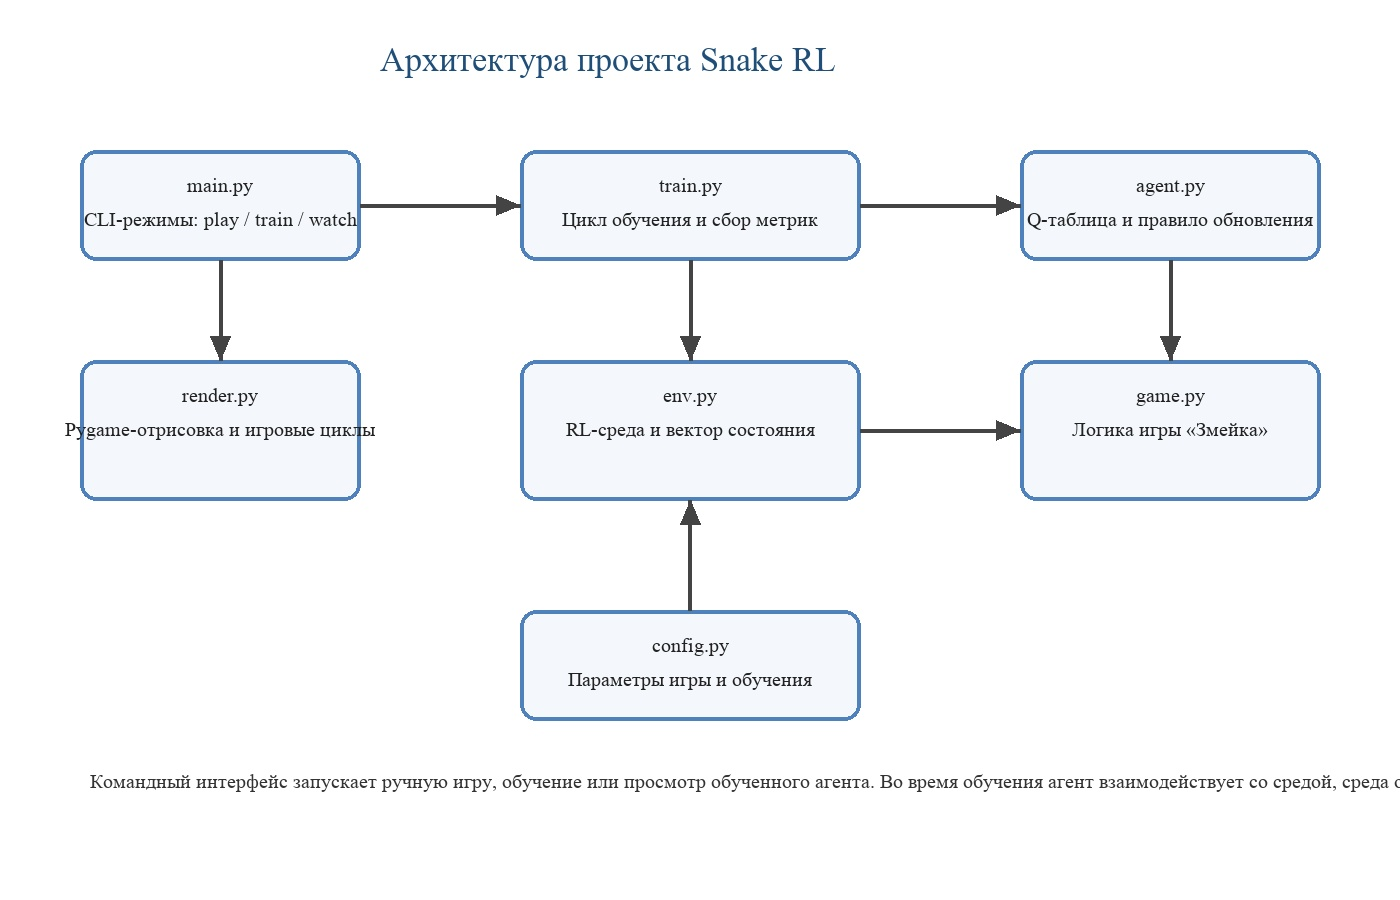
\includegraphics[width=0.82\textwidth]{architecture.jpg}

\end{frame}

% ═══════════════════════════════════════════════════════════════
%  SLIDE 7 — Q-learning Algorithm
% ═══════════════════════════════════════════════════════════════
\begin{frame}[t,shrink=5]{Алгоритм Q-learning}

\begin{center}
\card{0.85\textwidth}{%
\centering
\vspace{4pt}
{\Large $Q(s,a) \;\leftarrow\; Q(s,a) + \alpha\bigl[\,r + \gamma\,\max_{a'}Q(s',a') - Q(s,a)\,\bigr]$}
\vspace{4pt}
}
\end{center}

\vspace{0.3cm}
\centering
\textcolor{textsub}{\small ГИПЕРПАРАМЕТРЫ}\\[6pt]
\renewcommand{\arraystretch}{1.3}
\begin{tabular}{cccc}
    \arrayrulecolor{ruleclr}
    \toprule
    $\alpha$ & $\gamma$ & $\varepsilon_{0}$ & decay \\
    \midrule
    \textbf{0.1} & \textbf{0.9} & \textbf{1.0} & \textbf{0.995} \\
    \bottomrule
\end{tabular}
\renewcommand{\arraystretch}{1.0}

\vspace{0.3cm}
$\varepsilon$-жадная стратегия: \quad
\accenttag{$\varepsilon$: 1.0 $\rightarrow$ 0.05} \quad
{\small баланс исследования и использования}
\end{frame}

% ═══════════════════════════════════════════════════════════════
%  SLIDE 8 — Interface Screenshots
% ═══════════════════════════════════════════════════════════════
\begin{frame}{Интерфейс программы}

\centering
\begin{columns}[c]
\column{0.30\textwidth}
\centering
\fcolorbox{ruleclr}{surfacebg}{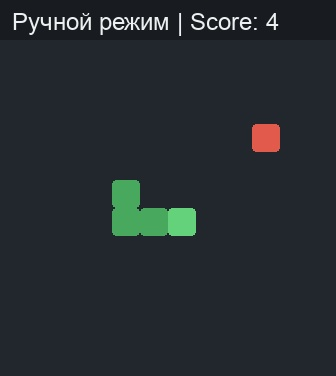
\includegraphics[width=0.94\textwidth]{manual_game.jpg}}
\vspace{4pt}\\
\textcolor{textsub}{\small Ручная игра}

\column{0.30\textwidth}
\centering
\fcolorbox{ruleclr}{surfacebg}{
\includegraphics[width=0.94\textwidth]{agent_mode.jpg}}
\vspace{4pt}\\
\textcolor{textsub}{\small Режим агента}

\column{0.30\textwidth}
\centering
\fcolorbox{ruleclr}{surfacebg}{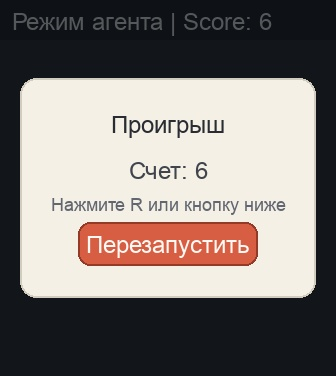
\includegraphics[width=0.94\textwidth]{game_over_modal.jpg}}
\vspace{4pt}\\
\textcolor{textsub}{\small Game over}
\end{columns}

\end{frame}

% ═══════════════════════════════════════════════════════════════
%  SLIDE 9 — Experiment Setup
% ═══════════════════════════════════════════════════════════════
\begin{frame}[shrink=12]{Методика эксперимента}

\vspace{0.2cm}
\centering
\begin{tikzpicture}[
    stepbox/.style={rounded corners=8pt, fill=accentlight, draw=none,
                 minimum width=2.8cm, minimum height=1.3cm, font=\normalsize,
                 text=textmain, align=center},
  ]
  \node[stepbox] (s1) at (0,0)   {\textbf{5}\\[-2pt]{\scriptsize запусков}};
  \node[font=\large,text=accent] at (2.0,0) {$\times$};
  \node[stepbox] (s2) at (4.0,0) {\textbf{8}\\[-2pt]{\scriptsize вариантов}};
  \node[font=\large,text=accent] at (6.0,0) {$\times$};
  \node[stepbox] (s3) at (8.0,0) {\textbf{100}\\[-2pt]{\scriptsize тестовых игр}};
\end{tikzpicture}

\vspace{0.3cm}
\begin{columns}[T]
\column{0.45\textwidth}
\textcolor{textsub}{\small ЭПИЗОДЫ ОБУЧЕНИЯ}\\[4pt]
50, 100, 200, 300, 500, 800, 1000, 1200

\column{0.45\textwidth}
\textcolor{textsub}{\small МЕТРИКА}\\[4pt]
Средний score на 100 тестовых играх\\(без исследования, $\varepsilon=0$)
\end{columns}
\end{frame}

% ═══════════════════════════════════════════════════════════════
%  SLIDE 10 — Results Chart
% ═══════════════════════════════════════════════════════════════
\begin{frame}{Результаты обучения}

\centering
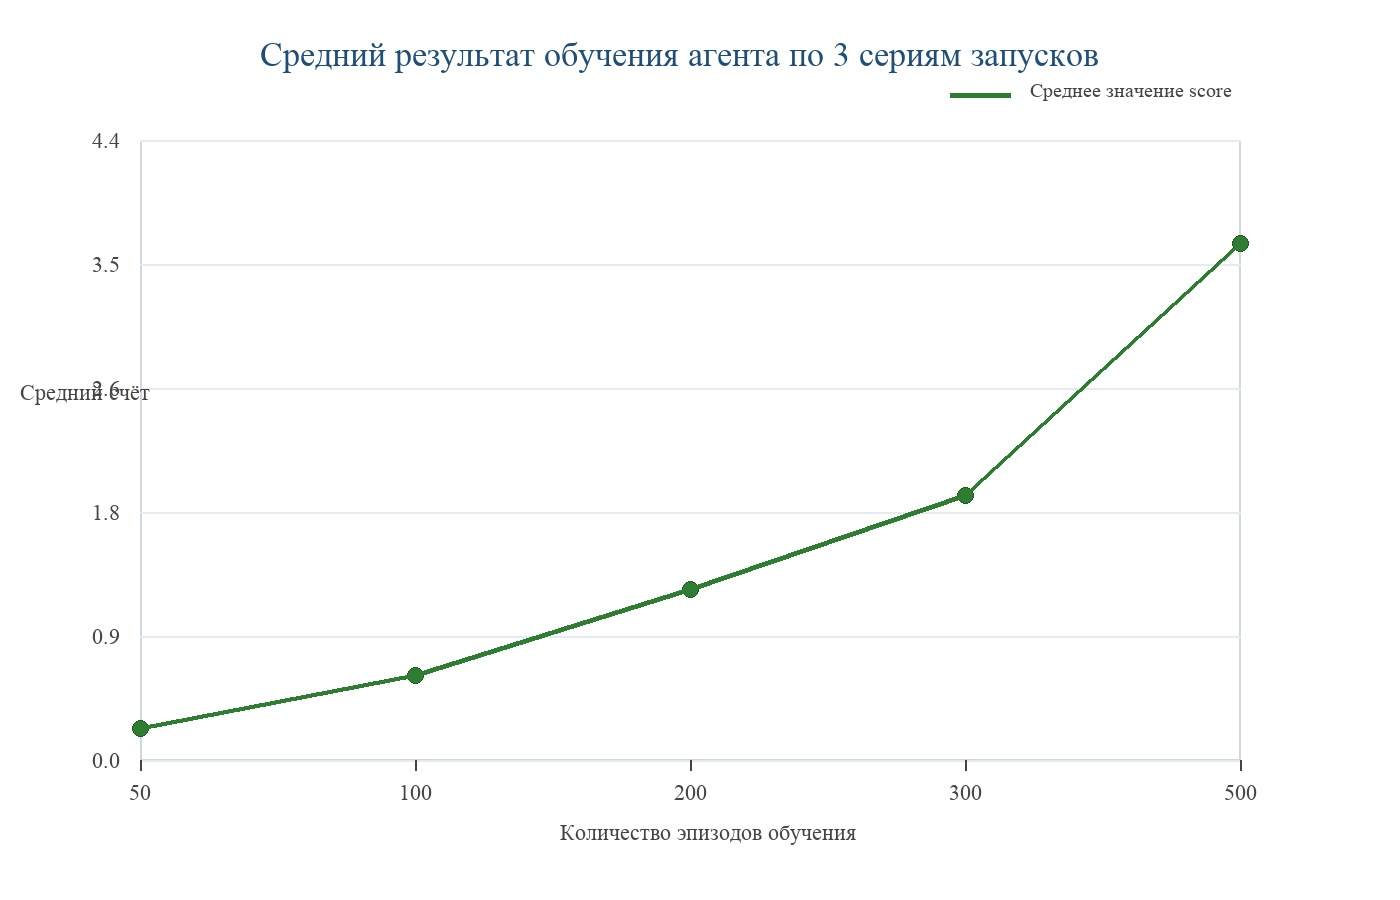
\includegraphics[width=0.78\textwidth]{learning_chart.jpg}

\end{frame}

% ═══════════════════════════════════════════════════════════════
%  SLIDE 11 — Results Table
% ═══════════════════════════════════════════════════════════════
\begin{frame}[t,shrink=3]{Рост качества игры}

\centering
\renewcommand{\arraystretch}{1.45}
\begin{tabular}{ccc}
    \arrayrulecolor{ruleclr}
    \toprule
    \textcolor{textsub}{\small Эпизоды} & \textcolor{textsub}{\small Средний score} & \textcolor{textsub}{\small Лучший score} \\
    \midrule
    50   & 4.26           & 15.80 \\
    100  & 7.54           & 19.20 \\
    500  & 13.96          & 21.40 \\
    \rowcolor{accentlight}
    1200 & \textbf{16.23} & \textbf{21.60} \\
    \bottomrule
\end{tabular}
\renewcommand{\arraystretch}{1.0}

\vspace{0.4cm}
\begin{columns}[c]
\column{0.45\textwidth}
\centering
\card{0.9\linewidth}{%
  \centering
  {\small Средний score}\\[2pt]
  {\LARGE\textcolor{accent}{\textbf{4.26}} {\normalsize$\rightarrow$} \textcolor{accent}{\textbf{16.23}}}%
}

\column{0.45\textwidth}
\centering
{\small После 800 эпизодов рост замедляется $\Rightarrow$ выход на плато}
\end{columns}
\end{frame}

% ═══════════════════════════════════════════════════════════════
%  SLIDE 12 — Conclusions
% ═══════════════════════════════════════════════════════════════
\begin{frame}{Выводы}

\vspace{0.2cm}
\begin{itemize}
    \setlength\itemsep{0.4cm}
    \item[\textcolor{successclr}{\textbullet}] Цель достигнута: игра реализована, агент обучен, результаты проанализированы
    \item[\textcolor{successclr}{\textbullet}] Табличный Q-learning формирует эффективную стратегию без нейросетей
    \item[\textcolor{successclr}{\textbullet}] 11 бинарных признаков --- компромисс между простотой и информативностью
    \item[\textcolor{accent}{\textbullet}] Перспективы: влияние гиперпараметров, DQN для сложных состояний
\end{itemize}

\vspace{0.4cm}
\centering
\textcolor{textsub}{\small Спасибо за внимание}

\end{frame}

\end{document}
